

\chapter{Marco Te\'orico}
\label{cap:preliminares}

\section{Impresión 3D}

 A diferencia de las técnicas principales que se emplean desde hace algunos años en la fabricación de objetos, que se encargan de sustraer, combinar, o deformar paulatina y controladamente materia hasta llegar a una pieza final, la impresión 3D funciona de un modo completamente distinto. La pieza se crea en un solo paso, capa por capa, a un ritmo medio de uno a dos centímetro de altura por hora; el objeto creado puede constar de mecanismos internos (como rodamientos de bolas), formas tejidas y entrelazadas, o incluso huecos y curvas \citep{Berchon2014}. Pues bien, todas las impresoras 3D, están basadas sobre el mismo principio: un modelo digital es transformado a un objeto físico de 3 dimensiones por adición de material en capas. Esto se conoce alternativamente como \textit{Manufactura Aditiva} \citep{tresdhub2018}. Este tipo de fabricación también se puede englobar dentro de lo que se denomina \textit{Fabricación digital}, cuyo principio básico es la transformación de la información  desde el mundo físico al digital. Según \citep{jorquera2016}, la fabricación digital incluye los siguientes sistemas y tecnologías:\\
 
 \begin{enumerate}
 	
	\item Sistemas integrados: Es un \textit{hardware} electrónico diseñado específicamente para llevar a cabo una o pocas tareas definidas. Las impresoras llevan un sistema electrónico integrado que utilizan para controlar los motores paso a paso que alimentan el papel, recibir información de los sensores de temperatura y finales de carrera, o que mandan al cabezal de impresión.
	\item Sistemas CNC (\textit{Computer Numeric Control} - control numérico computarizado): Es el control numérico de un sistema de automatización que se utiliza para controlar diferentes máquinas herramienta. Este sistema ha revolucionado la industria gracias a la simplificación del \textit{software} de diseño en conjunto con los lenguajes de programación como el \textit{.gcode}. Esencialmente, un sistema CNC es cualquier sistema que utiliza un ordenador para controlar los movimientos de una máquina.
	\item Software CAD (\textit{Computer Aided Design}- diseño asistido por computador): es, en esencia, un programa que sirve para la creación, edición análisis y visualización de modelos tridimensionales.  
	\item Internet: Los programas CAD actuales disponen de herramientas de trabajo colaborativo en red, de esta manera se define el producto y el proceso de fabricación de forma simultánea.\\

  \end{enumerate}

En la misma línea, y dependiendo de la profundidad técnica que el proceso de fabricación necesite, se agregan los sistemas \citep{leao2017}:

\begin{enumerate}
	\item Software CAE (\textit{Computer Aided Engineering} - Ingeniería Asistida por computador): Son los programas mayoritariamente usados para las tareas de análisis de ingeniería. Estos \textit{softwares}, a través de métodos numéricos como el método de elementos finitos o dinámica de fluidos computacional, se utilizan para, por ejemplo, analizar la robustez y el funcionamiento de ensambles de piezas.
	\item Software CAM (\textit{Computer Aided Manufacturing}- Manufactura Asistida por computador): Corresponde a programas que controlan las herramientas de máquinas de control numérico relacionadas con el proceso de manufactura a realizar, generando un código específico para el producto a fabricar. 

\end{enumerate}

%Figura: Expectativas impresi\'on 3D 
\begin{figure}[tp]
  \centering
    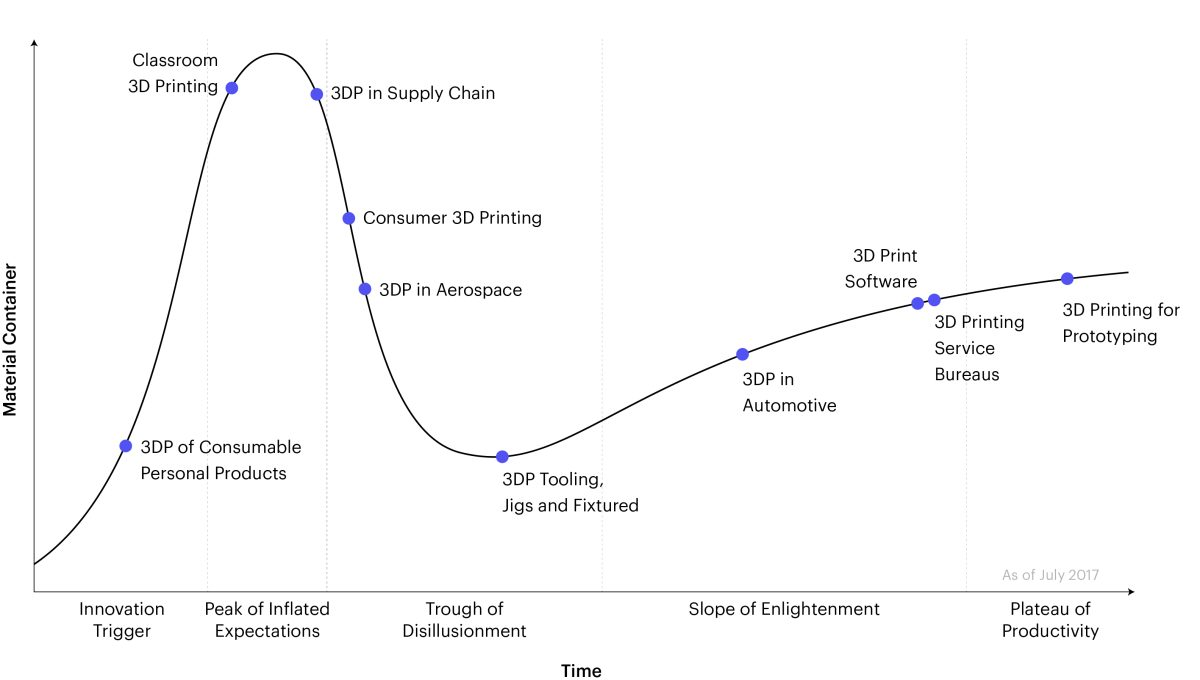
\includegraphics[width=\textwidth]{images/The3Dprintinghypecycle.png}
  \caption{Mi Figura}
  \label{fig:ejemplo}
\end{figure}

% Figura: \'Arbol XML 1
%\begin{figure}[tp]
%  \centering
%  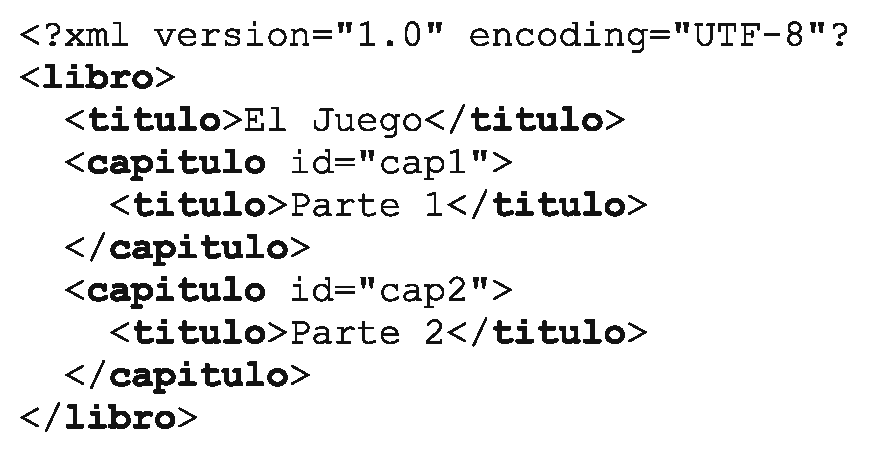
\includegraphics[scale=.5]{images/XML-document-example1}
%  \caption{\em Modelo de árbol para un documento XML.}
%  \label{fig:xml-tree-exa1}
%\end{figure}


\subsection{Historia de la impresión 3D}

El comienzo de la generación del concepto de impresión 3D puede ser rastreado al año 1976, a partir de la creación de la primera impresora a tinta por inyección \citep{maxey2013}. La utilización de la inyección de tinta abrió la pregunta respecto a qué tipo de materiales podían ser utilizados con esta tecnología, y cómo los mecanismos presentes en la época podían ser adaptados para abrir la posibilidad de ocupar otras materias primas. En Mayo de 1981, el Dr. Hideo Kodama del Instituto de Investigación Industrial del Municipio de Nagoya publicó detalles relativos a la técnica de prototipado rápido. Esta investigación se considera como la primera publicación que describe la técnica de fabricación capa a capa propia de los procesos de impresión 3D; no obstante, los desarrollos de Kodama no llegaron a ser materializados debido a problemas encontrados en el proceso de fundido de material. \citep{tresdsourced2020}. Paralelamente, la idea de ``máquinas de prototipado rápido'' continuó su desarrollo en Francia, por Jean-Claude André, Oliver de Witte y Alain le Méhauté. En la primera mitad de la década de los 80, le Méhauté investigaba en la empresa Alcatel sobre partes y piezas generadas a partir de la geometría fractal, y la manera en que éstas podrían ser fabricadas dada su complejidad de forma.
De Witte, quien era también investigador de Alcatel en el área de luz láser, propuso a le Méhauté que algunos líquidos compuestos por ciertos monómeros podían ser curados y transformados en sólidos tras la aplicación de luz láser, convirtiéndose en el primer paso para la construcción efectiva de máquinas de prototipado rápido a través de el proceso de Estereolitografía. Ambos compartieron el resultado de sus avances con André, que en ese tiempo trabajaba en el Centro Nacional Frances de Investigación Científica, para ya el año 1984 inscribir la patente de su desarrollo. Infortunadamente, el grupo debe abandonar el proyecto debido a problemas con la solidificación del material y poca rentabilidad desde la perspectiva económica \citep{alltresdp2018}.\

Con solo tres semanas de diferencia respecto a los investigadores franceses, Charles `Chuck' Hull solicita la patente del proceso de Esterolitografía con nuevos avances, como la utilización del formato STL (Standard Triangle Language) y la laminación digital de objetos. A diferencia del a Esterolitografía francesa, el método de Hull utiliza luz ultravioleta para el curado de fotopolímeros. El año 1986, obtenida su patente, Hull forma la empresa \textit{3D Systems} y lanza la primera impresora 3D, la \textit{SLA-1}, el año 1987 \citep{tresdsourced2020}.


\subsection{Métodos de impresión 3D}

\subsection{Impresoras 3D FDM}

\subsection{Tipologías de impresión 3D FDM}

\section{Mantenimiento}

\subsection{Historia y evolución del mantenimiento}

Si bien no existe precisión histórica o documentación para establecer los orígenes del mantenimiento ya sea, por ejemplo, en la diferencia entre la evolución de las distintas industrias, la literatura sí genera distintos consensos en lo que respecta a ciertos hitos que pueden dar luces a este contexto histórico. En este sentido, las principales referencias que existen en diversas fuentes bibliográficas sobre los tipos de mantenimiento llevados a cabo han concluido, de común acuerdo entre muchos autores, en establecer durante el siglo XX tres grandes etapas que, aunque no tienen una una frontera clara desde el punto de vista temporal, si pueden dar una clara idea de cómo ha sido la evolución de las técnicas y organizaciones que se han implementado durante dicho siglo. Se ha convenido entonces, que la evolución del mantenimiento ha tenido tres etapas, a las cuales se les denomina \textit{primera, segunda} y \textit{tercera generación} \citep{gonzalez2005}.
Así, el comienzo del siglo XX marca efectivamente el inicio de las actividades de mantenimiento reparativo y la creación de los primeros talleres que originan la \textit{Primera Generación} del mantenimiento, que se extiende hasta mediados del siglo y tiene como características relevantes \citep{garcia2012}:

\begin{itemize}
\item Equipos robustos, sobredimensionados y simples.
\item Volúmenes de producción bajos.
\item Las actividades demandaban poca destreza.
\item No existía la alta mecanización industrial
\item Poca importancia a los tiempos de parada de los equipos.
\item La prevención de fallas en los equipos no era prioridad.
\item El mantenimiento era mantenimiento reactivo o de reparación.
\item No había necesidad de un mantenimiento sistemático.
\end{itemize}  

Esta etapa, la más larga desde la revolución industrial hasta después de la Segunda Guerra Mundial, se caracteriza esencialmente por la corrección de averías, reengrases, lubricaciones y limpiezas \citep{gonzalez2005}.

En tiempos posteriores a la guerra se vio la necesidad de implantar técnicas con el fin de prevenir las fallas de los equipos en combate y disminuir los costos de reparación, por lo que vino a tomar importancia relevante la disponibilidad y duración de vida útil de la maquinaria \citep{garcia2012}. El descubrimiento de relación entre edad de equipos y probabilidad de fallos, junto a la enorme competencia industrial, además de la incorporación de los fabricantes orientales al mundo competitivo occidental, es uno de los desencadenantes de una contínua búsqueda de mejores resultados. En esta etapa denominada \textit{segunda generación}, se ponen en marcha sistemas de mantenimiento preventivo basados en revisiones cíclicas de equipos, instalaciones y medios en general \citep{gonzalez2005}. Dentro de las características principales de este periodo se señalan \citep{garcia2012}:

\begin{itemize}
\item Importancia de la productividad
\item Incremento de la mecanización en las industrias
\item Aumento de la complejidad de los equipos
\item Mayor interés a los tiempos de parada de los equipos
\item Inicio del mantenimiento preventivo
\item Altos niveles de inventario de repuestos
\item Crecimiento de los costos de mantenimiento
\item Sistemas de planificación y control de mantenimiento
\item Aumento de la vida útil de los equipos y sistemas
\item Inicio de la sistematización del Mantenimiento
\end{itemize}

La optimización de este mantenimiento de segunda generación, basado por tanto en mantenimientos preventivos rutinarios y mantenimiento correctivo, se fundamenta en avanzados sistemas de planificación de actividades y de control de trabajos realizados; entendiendo por control tanto el lanzamiento de órdenes de trabajo como la retroalientacnión y verificación de los datos habidos en esas órdenes de trabajo \citep{gonzalez2005}.

Se debe decir que, durante el periodo posterior a 1980, se han visto los peores accidentes en la historia de la industria mundial. Las filtraciones de baterías en Bhopal, India, o  la amenaza a la supervivencia de la humanidad causada por el accidente nuclear de Chernobyl, solo han hecho que la industria manufacturera realcen la importancia del mantenimiento \citep{shenoy2005}. Este punto de inflexión, sumado a las preocupaciones que ya existían ciertos postulados en relación a la máxima calidad, seguridad y protección del medio ambiente, dio origen a la tercera generación del mantenimiento, que se extendió hasta el final del siglo \citep{garcia2012}. Cabe destacar que en el mantenimiento de tercera generación, la observancia de normativa adquiere una importancia primordial. Son muchas las administraciones estatales, autonómicas y locales que abordan reglamentaciones específicas del mantenimiento; así pues, aparecen reglamentos para aparatos a presión, equipos de manutención y transporte, ascensores y escaleras mecánicas, etc. Este aspecto toma también relevancia y define lo que se ha convenido en llamar, dentro de los mantenimientos preventivos, mantenimientos legales o reglamentarios \citep{gonzalez2005}.    



\subsection{Mantenimiento correctivo}

\subsection{Mantenimiento preventivo}

\subsection{Mantenimiento centrado en la condición}

\subsection{Mantenimiento centrado en la confiabilidad}


\subsection{Confiabilidad}

La confiabilidad puede ser definida como la "confianza que se tiene de que un componente, equipo o sistema desempeñe su función básica, durante un periodo de tiempo preestablecido, bajo condiciones estándares de operación; otra definición es la probabilidad de que un ítem pueda desempeñar su función requerida durante un intervalo establecido y bajo condiciones de uso definidas \citep{dairo2016}. Esta segunda definición da a entender que existen herramientas estadísticas que pueden ser utilizadas para obtener información acerca del cómo se comportan las fallas en el tiempo.

\subsubsection{Función densidad de probabilidad}

La función densidad de probabilidad puede describir la distribución de la probabilidad de una variable aleatoria continua $X$. Así, una función de densidad de probabilidad es una función tal que:


 $$f(x)\geqslant 0$$
 $$\int_{-\infty}^{\infty}f(x)dx=1$$
 \begin{equation*}
 P(a\geqslant X \geqslant b)=\int_{a}^{b}f(x)dx= \text{ área bajo } f(x) \text{ de } a \text{ a } b, \text{ para cualquier } a \text{ y } b.
 \end{equation*}



Esta función proporciona una descripción simple de las probabilidades asociadas a una variable aleatoria.
\subsubsection{Media y varianza de una variable continua}

Si se tiene que $X$ es una variable aleatoria continua con función de densidad de probabilidad $f(x)$, se define la Media de $X$ como:

\begin{equation*}
\mu=E(X)=\int_{-\infty}^{\infty}xf(x)dx
\end{equation*}

Asimismo, la Varianza de $X$:

\begin{equation*}
\sigma^2=V(X)=\int_{-\infty}^{\infty}(x-\mu)^{2}f(x)dx=\int_{-\infty}^{\infty}x^{2}f(x)dx-\mu^2
\end{equation*}

La Desviación Estandar:

\begin{equation*}
\sigma=\sqrt{V(X)}
\end{equation*}

\subsubsection{Distribución normal}

Variables aleatorias con medias y varianzas diferentes pueden modelares por medio de funciones de densidad de probabilidad normal, con la elección adecuada del centro y anchura de la curva. La función de densidad de probabilidad normal se define como:

\begin{equation*}
f(x)=\frac{1}{\sqrt{2\pi\sigma}}e^{\frac{-(x-\mu)^2}{2\sigma^2}}  ,  -\infty<x<\infty
\end{equation*}

tiene una distribución normal con parámetros $\mu$, donde $-\infty<\mu<\infty$, y $\sigma>0$.\\

Además,
\begin{equation*}
E(X)=\mu , V(x)=\sigma^2
\end{equation*}

\subsubsection{Distribución exponencial}

La distribución exponencial debe su nombre a la función exponencial de la función de densidad de probabilidad. Así, la variable aleatoria $X$ (que es igual a la distancia entre conteos sucesivos de un proceso de Poisson con media $\lambda>0$ tiene una distribución exponencial con parámetro $\lambda$:

\begin{equation*}
f(x)=\lambda e^{-\lambda x}, 0<x<\infty
\end{equation*}

Si la variable tiene una distribución exponencial con parámetro $\lambda$:

\begin{equation*}
E(x)=\frac{1}{\lambda}, V(X)=\frac{1}{\lambda^2}
\end{equation*}

\subsubsection{Distribución de Weibull}

La distribución de Weibull se utiliza con frecuencia para modelar el tiempo hasta que ocurre una falla en algún sistema. La variable aleatoria $X$ con función de densidad de probabilidad:

\begin{equation*}
f(x)=\frac{\beta}{\delta}\left( \frac{x}{\delta} \right)^{\beta-1}e^{\left( \frac{x}{\delta} \right)}{}^\beta
\end{equation*}

tiene una distribución de Weibull con parámetro de escala $\delta>0$ y parámetro de forma $\beta>0$.


\section{Lean Manufacturing}

\subsection{Historia Lean Manufacturing}

\subsection{Herramientas de mantenimiento}

\section{Design Thinking}

\subsection{Metodologías ágiles}

\subsection{Design Thinking}

\subsection{Fases del Design Thinking}


\section{Herramientas de software}

\subsection{Lenguajes de programación orientada a objetos}

\subsection{Lenguajes de hojas de estilo}

\subsection{Bases de datos}

\subsection{Arquitectura Cliente-Servidor}

\subsection{API}

\subsection{Ordenadores de placa reducida}



 

% Figura: \'Arbol XML 1
%\begin{figure}[tp]
%  \centering
%  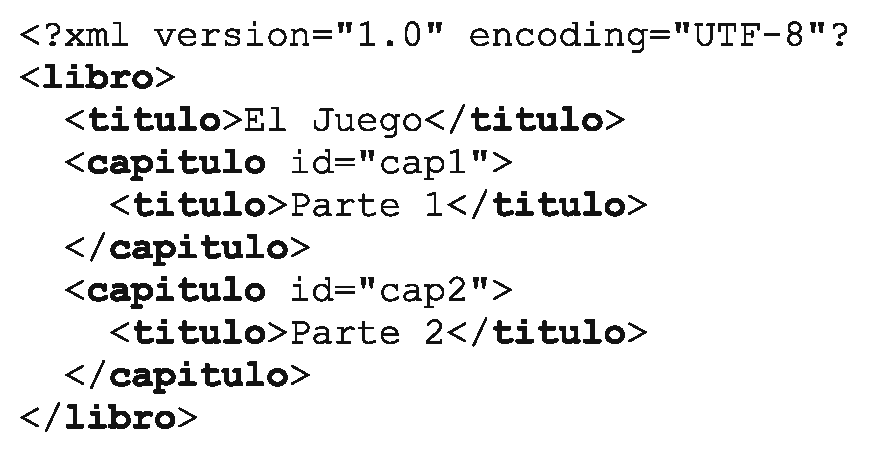
\includegraphics[scale=.5]{images/XML-document-example1}
%  \caption{\em Modelo de árbol para un documento XML.}
%  \label{fig:xml-tree-exa1}
%\end{figure}



